\documentclass[../../main.tex]{subfiles}
\begin{document}

{\bf [解]}

$\alpha = x + y, \beta = xy$ とすると，実数$x, y$が存在する条件は，$x, y$を解に持つ二次方程式$t^2 -\alpha t + \beta = 0$の判別式が非負であることで，
\begin{align}
 \alpha^2 - 4\beta \ge 0 \label{eq:1}
\end{align}
である．また題意の条件$x^2+y^2=a^2$から
\begin{align}
 \alpha^2 - 2\beta = a^2 \quad \dots \text{③} \label{eq:2} 
\end{align}
である．
$u, v$を$\alpha,\beta$で表すと
\begin{align}
u = \alpha + 1, \quad v = 1 - 2\beta \quad \dots \text{②} \\ 
\alpha = u - 1, \beta = \frac{1}{2}(1 - v) \label{eq:3} 
\end{align}
である．
\cref{eq:1,eq:2}の元で\cref{eq:3}の通る領域を求める．
\cref{eq:3}を\cref{eq:1,eq:2}に代入して
\begin{align}
\begin{cases}
(u-1)^2 - 2(1-v) \ge 0 \\
(u-1)^2 - (1-v) = a^2
\end{cases}
\iff
\begin{cases}
v \ge \frac{1}{2}(-u^2 + 2u + 1) \\
v = -u^2 + 2u + a^2
\end{cases} \label{eq:4}
\end{align}
が求める$(u,v)$の方程式である．

\noindent
(2) 
$a$が
\begin{align}
 \frac{1}{\sqrt{2}} \le a \le 1
\end{align}
の範囲を動く時，
\begin{align}
 \frac{1}{2} \le a^2 \le 1
\end{align}
だから，\cref{eq:4}の領域は
\begin{align}
\begin{cases}
-u^2 + 2u + \frac{1}{2} \le v \le -u^2 + 2u + 1 \\
v \ge \frac{1}{2}(-u^2 + 2u + 1)
\end{cases} \label{eq:5}
\end{align}
となる．これを図示すると下図斜線部（境界含む）である．
境界の方程式は
\begin{align}
 \begin{cases}
  v = -u^2 + 2u + \frac{1}{2} \\
  v = -u^2 + 2u + 1 \\
  v = \frac{1}{2}(-u^2 + 2u + 1)
 \end{cases}
\end{align}
である．

\begin{figure}[htb]
\begin{center}
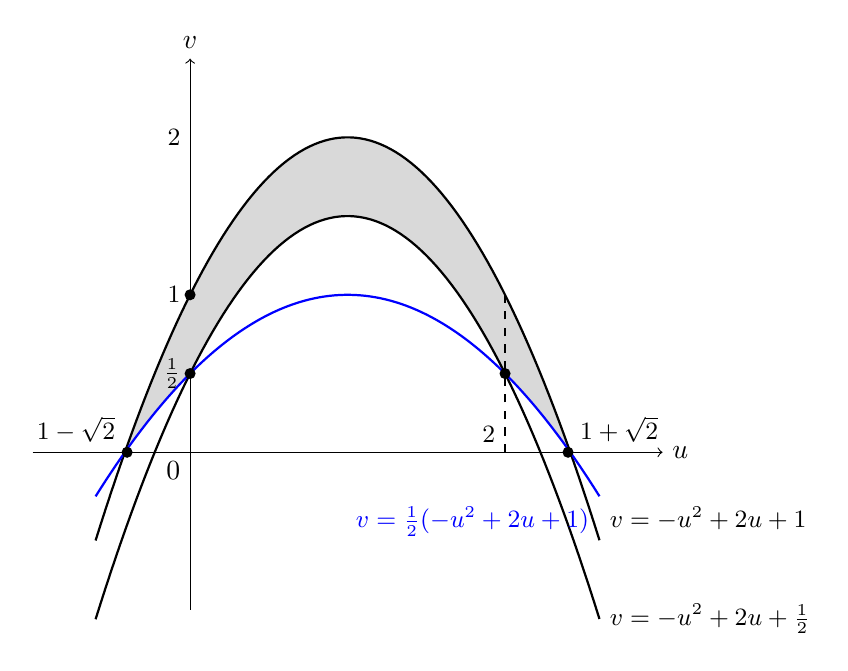
\begin{tikzpicture}[scale=2]
  \draw[->] (-1,0) -- (3,0) node[right] {$u$};
  \draw[->] (0,-1) -- (0,2.5) node[above] {$v$};
  \node[below left] at (0,0) {$0$};

  % 塗りつぶし
  \fill[gray!30, domain=0:2, samples=50]
    plot (\x, {-\x*\x + 2*\x + 1})
    -- plot[domain=2:0] (\x, {-\x*\x + 2*\x + 0.5})
    -- cycle;

  %塗りつぶし2 
  \fill[gray!30, domain=2:2.414, samples=50]
    plot (\x, {-\x*\x + 2*\x + 1})
    -- plot[domain=2.414:2.0] (\x, {-0.5*\x*\x + \x + 0.5})
    -- cycle;

  %塗りつぶし3
  \fill[gray!30, domain=-0.414:0, samples=50]
    plot (\x, {-\x*\x + 2*\x + 1})
    -- plot[domain=0:-0.414] (\x, {-0.5*\x*\x + \x + 0.5})
    -- cycle;

  \draw[thick, domain=-0.6:2.6, samples=100] plot (\x, {-\x*\x + 2*\x + 1}) node[above right] {\small $v = -u^2 + 2u + 1$};
  \draw[thick, domain=-0.6:2.6, samples=100] plot (\x, {-\x*\x + 2*\x + 0.5}) node[right] {\small $v = -u^2 + 2u + \frac{1}{2}$};
  \draw[thick, blue, domain=-0.6:2.6, samples=100] plot (\x, {-0.5*\x*\x + \x + 0.5}) node[below left] {\small $v = \frac{1}{2}(-u^2 + 2u + 1)$};

  \node[left, font=\small] at (0,1) {$1$};
  \node[left, font=\small] at (0,0.5) {$\frac{1}{2}$};
  \node[left, font=\small] at (0,2) {$2$};
  \node[above left, font=\small] at (2,0) {$2$};
  \node[above left, font=\small] at (-0.414,0) {$1-\sqrt{2}$};
  \node[above right, font=\small] at (2.414,0) {$1+\sqrt{2}$}; % 1 \pm \sqrt{2}


  % 補助線
  \draw[dashed, thin] (2, 0) -- (2, 1);


  \fill (0,1) circle (1pt);
  \fill (0,0.5) circle (1pt);
  \fill (2,0.5) circle (1pt);
  \fill (-0.4,0) circle (1pt);
  \fill (2.4,0) circle (1pt);
\end{tikzpicture}
\end{center}
\caption{条件を満たす$(u,v)$の範囲（斜線部境界含む）}
\end{figure}

\end{document}
